\section{Exercise 3.10\footnote{Exercises from the reference book: Sipser M.,
\emph{Introduction to the Theory of Computation}, 3rd edition (2013).}}

\subsection{Introductory remarks}
In the standard definition of the Turing machine (\TM{}), each step writes a symbol to
the cell pointed by the head. Here, we consider that writing the same symbol as
the one that is already in this cell does not count as ``writing''. We
interpret ``writing to a cell'' as altering the content of the cell
(see~\ref{writing}).
\begin{figure}
    \centering
    \begin{subfigure}{0.4\textwidth}
        \centering
		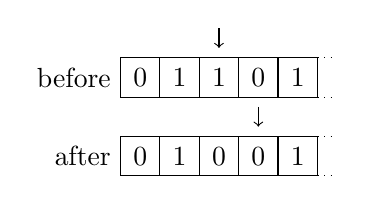
\begin{tikzpicture}[scale=.5]
			\draw[->] (3,3.25) -- (3,2.75) ;
			\draw[->] (4,1.25) -- (4,.75) ;

			\foreach \y/\v in {2/{1/0,2/1,3/1,4/0,5/1},0/{1/0,2/1,3/0,4/0,5/1}}
			\foreach \x/\k in \v {%
				\draw (\x,\y) +(-.5,-.5) rectangle ++(.5,.5);
				\draw (\x,\y) node{$\k$};
			}

			\draw[dotted] (5.5,2.5) -- (6,2.5);
			\draw[dotted] (5.5,1.5) -- (6,1.5);
			\draw[dotted] (5.5,.5) -- (6,.5);
			\draw[dotted] (5.5,-.5) -- (6,-.5);

			\draw (.5,2) node[anchor=east]{before} ;
			\draw (.5,0) node[anchor=east]{after} ;

		\end{tikzpicture}
        \caption{Altering a cell, \(\delta(q_i,1) = (q_j,0,R)\). Counting as one write operation.}
    \end{subfigure}%
    \begin{subfigure}{0.4\textwidth}
        \centering
		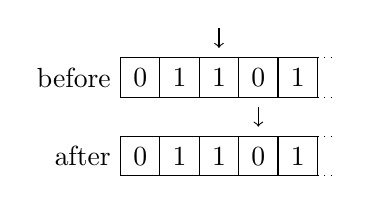
\begin{tikzpicture}[scale=.5]
			\draw[->] (3,3.25) -- (3,2.75) ;
			\draw[->] (4,1.25) -- (4,.75) ;

			\foreach \y/\v in {2/{1/0,2/1,3/1,4/0,5/1},0/{1/0,2/1,3/1,4/0,5/1}}
			\foreach \x/\k in \v {%
				\draw (\x,\y) +(-.5,-.5) rectangle ++(.5,.5);
				\draw (\x,\y) node{$\k$};
			}

			\draw[dotted] (5.5,2.5) -- (6,2.5);
			\draw[dotted] (5.5,1.5) -- (6,1.5);
			\draw[dotted] (5.5,.5) -- (6,.5);
			\draw[dotted] (5.5,-.5) -- (6,-.5);

			\draw (.5,2) node[anchor=east]{before} ;
			\draw (.5,0) node[anchor=east]{after} ;

		\end{tikzpicture}
		\caption{Keeping the cell as is, \(\delta(q_i,1) = (q_j,1,R)\). Counting as zero write operations.}
    \end{subfigure}
	\caption{Counting write operations.}\label{writing}
\end{figure}

At the beginning of the execution of the \TM{}, the input is
present on the tape and this counts as zero write operations.

If some set/combinations/thing is of finite size and does not depend on the input
we can encode all its different ``elements'' in the states of the \TM{}.
In particular, states can be tuples and remember as many pieces of
information we want to as long as their size is fixed (independent of the
input size).

We call the simulated \TM{} (the one we want to simulate) \(M\) and we
call the simulation \TM{} (the one used to simulate \(M\)) \(S\).

When we say that we add new symbols (\X{}, \e{}) we suppose they
are not already part of some used alphabet and this is without loss of
generality.
Similarily, we make the blank symbol of the simulated \TM{} and the
simulation \TM{} different. The blank symbol of \(M\)
is \°{} while the blank symbol of \(S\)
is \0{}. In general you can consider that the tape alphabet of \(M\)
does not include any of the symbols we will add to make \(S\) work.
For example, we can use one color for the tape alphabet of \(M\) and
another color for symbols we add. Here we will consider that all symbols used
by \(M\) are dotted (like \°{}) while the symbols that
have a special meaning for \(S\) are not (like \0{}).

Note that any transition that we do not define explicitely will be implicitely
defined as leading to the reject state.

Finaly, note that going left when the head points to the leftmost cell of the
tape means that we stay on the leftmost cell of the tape.

\subsection{Using two writes per cell}
The idea is to simulate each step of the simulated
\TM{} by copying all ``working'' cells to new (unused) cells
while applying the transition function to the cell pointed by the head.

We use a copy procedure that copies each character after
the other by doing ``zig-zags'' between the cells to be copied and the destination
cells. In order to remember which cells were already copied we cross those
cells off during the procedure.

We implement the cross off operation as
writing a special character (for example, \X{}) in the concerned cell.
This operation counts thus as one write operation. The cost of writing the
symbol of the copied cell to the destination also counts as a write. A cell
will thus be written to at most twice (once when copied to, and then
once when crossed off).

In order to detect when the copy procedure has copied all cells, we add a
special character (for example, \e)
at the end of the currently used portion of the tape.
We thus add this special symbol directly to the right of the last cell being written to by the
copy procedure (and also at the end of the input before beginning the
simulation). The cells containing this special character will only be written to once.
This is handled by steps 7 and 8 in~\ref{copying:last}.

Here are the detailed steps to copy a symbol \A{}:
\begin{enumerate}
	\item Cross off \A{} by writing a \X{}. This
		counts as a single write operation.
	\item Enter a state that remembers that we need to copy symbol
		\A{}, for example, \((\s,\e)\). We are allowed
		to do this since the alphabet of M is a finite set (and its size does not
		depend on the input).
	\item While in state \((\s,\e)\), move right (without
		altering the current cell) until we reach
		the symbol \e, change then to state
		\((\s,\0{})\).
	\item While in state \((\s,\0{})\), move right (without
	altering the current cell) until we reach the symbol \0{}.
	\item Replace the \0{} by \A{} using a
		single write operation and enter state \((\texttt{x})\).
	\item While in state \((\texttt{x})\), move left until we reach
		the symbol \X{}, enter state \((\texttt{?})\)
		then move right.
\end{enumerate}
A copy of all the cells can be achieved by entering state \((\texttt{?})\)
then apply the procedure above repeatedly.
The copy stops when in state \((\texttt{?})\) we read a \e{}
symbol (see~\ref{copying}).
\begin{figure}
    \centering
    \begin{subfigure}{0.4\textwidth}
        \centering
		\begin{tikzpicture}[scale=.5]
			\draw[->] (1,3.25) ++(0, 0)-- +(0,-.5) ;
			\draw[->] (1,3.25) ++(0,-2) -- +(0,-.5) ;
			\draw[->] (6,3.25) ++(0,-4) -- +(0,-.5) ;
			\draw[->] (7,3.25) ++(0,-6) -- +(0,-.5) ;
			\draw[->] (7,3.25) ++(0,-8) -- +(0,-.5) ;
			\draw[->] (2,3.25) ++(0,-10) -- +(0,-.5) ;

			\foreach \y/\v in {%
				2/{1/\Q,2/\A,3/\A,4/\Q,5/\A,6/\e,7/\0,8/\0,9/\0,10/\0,11/\0,12/\0},%
				0/{1/\X,2/\A,3/\A,4/\Q,5/\A,6/\e,7/\0,8/\0,9/\0,10/\0,11/\0,12/\0},%
				-2/{1/\X,2/\A,3/\A,4/\Q,5/\A,6/\e,7/\0,8/\0,9/\0,10/\0,11/\0,12/\0},%
				-4/{1/\X,2/\A,3/\A,4/\Q,5/\A,6/\e,7/\0,8/\0,9/\0,10/\0,11/\0,12/\0},%
				-6/{1/\X,2/\A,3/\A,4/\Q,5/\A,6/\e,7/\Q,8/\0,9/\0,10/\0,11/\0,12/\0},%
				-8/{1/\X,2/\A,3/\A,4/\Q,5/\A,6/\e,7/\Q,8/\0,9/\0,10/\0,11/\0,12/\0},%
			}{%
				\draw[dotted] (12.5,\y) +(0,0.5)-- +(.5,0.5);
				\draw[dotted] (12.5,\y) +(0,-.5)-- +(.5,-.5);
				\foreach \x/\k in \v {%
					\draw (\x,\y) +(-.5,-.5) rectangle ++(.5,.5);
					\draw (\x,\y) node{$\k$};
				}
			}

			\draw (.5,2) node[anchor=east]{1.} ;
			\draw (.5,0) node[anchor=east]{2.} ;
			\draw (.5,-2) node[anchor=east]{3.} ;
			\draw (.5,-4) node[anchor=east]{4.} ;
			\draw (.5,-6) node[anchor=east]{5.} ;
			\draw (.5,-8) node[anchor=east]{6.} ;

		\end{tikzpicture}
	\caption{Copying the first cell.}
    \end{subfigure}%
    \begin{subfigure}{0.4\textwidth}
        \centering
		\begin{tikzpicture}[scale=.5]
			\draw[->] (5,3.25) ++(0, 0)-- +(0,-.5) ;
			\draw[->] (5,3.25) ++(0,-2) -- +(0,-.5) ;
			\draw[->] (6,3.25) ++(0,-4) -- +(0,-.5) ;
			\draw[->] (11,3.25) ++(0,-6) -- +(0,-.5) ;
			\draw[->] (11,3.25) ++(0,-8) -- +(0,-.5) ;
			\draw[->] (6,3.25) ++(0,-10) -- +(0,-.5) ;
			\draw[->] (12,3.25) ++(0,-12) -- +(0,-.5) ;
			\draw[->] (12,3.25) ++(0,-14) -- +(0,-.5) ;
			\draw[->] (7,3.25) ++(0,-16) -- +(0,-.5) ;

			\foreach \y/\v in {%
				2/{1/\X,2/\X,3/\X,4/\X,5/\A,6/\e,7/\Q,8/\A,9/\A,10/\Q,11/\0,12/\0},%
				0/{1/\X,2/\X,3/\X,4/\X,5/\X,6/\e,7/\Q,8/\A,9/\A,10/\Q,11/\0,12/\0},%
				-2/{1/\X,2/\X,3/\X,4/\X,5/\X,6/\e,7/\Q,8/\A,9/\A,10/\Q,11/\0,12/\0},%
				-4/{1/\X,2/\X,3/\X,4/\X,5/\X,6/\e,7/\Q,8/\A,9/\A,10/\Q,11/\0,12/\0},%
				-6/{1/\X,2/\X,3/\X,4/\X,5/\X,6/\e,7/\Q,8/\A,9/\A,10/\Q,11/\A,12/\0},%
				-8/{1/\X,2/\X,3/\X,4/\X,5/\X,6/\e,7/\Q,8/\A,9/\A,10/\Q,11/\A,12/\0},%
				-10/{1/\X,2/\X,3/\X,4/\X,5/\X,6/\e,7/\Q,8/\A,9/\A,10/\Q,11/\A,12/\0},%
				-12/{1/\X,2/\X,3/\X,4/\X,5/\X,6/\e,7/\Q,8/\A,9/\A,10/\Q,11/\A,12/\e},%
				-14/{1/\X,2/\X,3/\X,4/\X,5/\X,6/\e,7/\Q,8/\A,9/\A,10/\Q,11/\A,12/\e},%
			}{%
				\draw[dotted] (12.5,\y) +(0,0.5)-- +(.5,0.5);
				\draw[dotted] (12.5,\y) +(0,-.5)-- +(.5,-.5);
				\foreach \x/\k in \v {%
					\draw (\x,\y) +(-.5,-.5) rectangle ++(.5,.5);
					\draw (\x,\y) node{$\k$};
				}
			}

			\draw (.5,2) node[anchor=east]{1.} ;
			\draw (.5,0) node[anchor=east]{2.} ;
			\draw (.5,-2) node[anchor=east]{3.} ;
			\draw (.5,-4) node[anchor=east]{4.} ;
			\draw (.5,-6) node[anchor=east]{5.} ;
			\draw (.5,-8) node[anchor=east]{6.} ;
			\draw (.5,-10) node[anchor=east]{7.} ;
			\draw (.5,-12) node[anchor=east]{8.} ;
			\draw (.5,-14) node[anchor=east]{9.} ;

		\end{tikzpicture}
	\caption{Copying the last cell.}\label{copying:last}
    \end{subfigure}
	\caption{Copying working cells.}\label{copying}
\end{figure}

We still need to describe how we can simulate \(M\), that is, remember the
current state of \(M\), remember the position of the head on the tape of \(M\),
update the cell pointed by the head and move the head according to the
transition function of \(M\).

To remember the current state $q_i$ of $M$,
we prepend the current state of $S$ with $q_i$ (for example replace
$(\s,\e)$ in the previous explanation by $(q_i,\s,\e)$).
To remember the position of the head of the simulated \TM{} we use
colored symbols $\HA$ (in addition to the color used to differentiate the symbols
used by \(M\) from the symbols having a special meaning for \(S\),
see~\ref{head}).
\begin{figure}
	\centering
	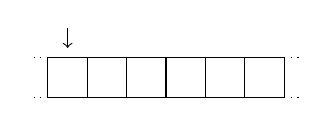
\begin{tikzpicture}[scale=.5]
		\draw[->] (1,3.25) -- (1,2.75) ;

		\foreach \y/\v in {2/{1/\Q,2/\HA,3/\Q,4/\Q,5/\A,6/\e}}
		\foreach \x/\k in \v {%
			\draw (\x,\y) +(-.5,-.5) rectangle ++(.5,.5);
			\draw (\x,\y) node{$\k$};
		}

		\draw[dotted] (0.5,2.5) -- (0,2.5);
		\draw[dotted] (0.5,1.5) -- (0,1.5);
		\draw[dotted] (6.5,2.5) -- (7,2.5);
		\draw[dotted] (6.5,1.5) -- (7,1.5);

	\end{tikzpicture}
	\caption{The first cell is pointed by the head of \(S\) (the arrow).
	The second cell is pointed by the head of \(M\) (the starred symbol).}\label{head}
\end{figure}
We do not need to color the first cell at the beginning of
the simulation since we ``know'' the first cell is pointed by the head at the
beginning. Again we can handle this using states since there is a finite number
of possibilities. A simple way to do this is to use special states for the
first steps of \(S\) that will allow us to copy the input with the
appropriate symbols/marks/colors added.

Before copying a cell we need to check whether the next one is the head (is a
colored symbol).
In that case, we have two possibilities (see~\ref{transition}):
\begin{enumerate}
\item If the transition function makes the head move left, then
we copy the current cell (the cell to the left of the
head) using the colored version of the symbol, write the symbol designated by
the transition function to the destination cell for the
cell pointed by the head, and then copy the cell to the right of the head
using the normal copy procedure.
\item If the transition function makes the head move right, then
we copy the current cell (the cell to the left of the
head) using the normal copy procedure, write the symbol designated by
the transition function to the destination cell for the
cell pointed by the head, and then copy the cell to the right of the head
using the colored version of the symbol.
\end{enumerate}
\begin{figure}
    \centering
    \begin{subfigure}{0.4\textwidth}
        \centering
		\begin{tikzpicture}[scale=.5]
			\draw[->] (2,3.25) ++(0, 0)-- +(0,-.5) ;
			\draw[->] (5,3.25) ++(0,-2) -- +(0,-.5) ;

			\foreach \y/\v in {%
				2/{1/\X,2/\Q,3/\HA,4/\A,5/\A,6/\e,7/\A,8/\0,9/\0,10/\0,11/\0,12/\0},%
				0/{1/\X,2/\X,3/\X,4/\X,5/\A,6/\e,7/\A,8/\HQ,9/\Q,10/\A,11/\0,12/\0},%
			}{%
				\draw[dotted] (12.5,\y) +(0,0.5)-- +(.5,0.5);
				\draw[dotted] (12.5,\y) +(0,-.5)-- +(.5,-.5);
				\foreach \x/\k in \v {%
					\draw (\x,\y) +(-.5,-.5) rectangle ++(.5,.5);
					\draw (\x,\y) node{$\k$};
				}
			}

			\draw (.5,2) node[anchor=east]{1.} ;
			\draw (.5,0) node[anchor=east]{2.} ;

		\end{tikzpicture}
		\caption{\(\delta(q_i,a) = (q_j,b,L)\), that is, moving left.}
    \end{subfigure}%
    \begin{subfigure}{0.4\textwidth}
        \centering
		\begin{tikzpicture}[scale=.5]
			\draw[->] (2,3.25) ++(0, 0)-- +(0,-.5) ;
			\draw[->] (5,3.25) ++(0,-2) -- +(0,-.5) ;

			\foreach \y/\v in {%
				2/{1/\X,2/\Q,3/\HA,4/\A,5/\A,6/\e,7/\A,8/\0,9/\0,10/\0,11/\0,12/\0},%
				0/{1/\X,2/\X,3/\X,4/\X,5/\A,6/\e,7/\A,8/\Q,9/\Q,10/\HA,11/\0,12/\0},%
			}{%
				\draw[dotted] (12.5,\y) +(0,0.5)-- +(.5,0.5);
				\draw[dotted] (12.5,\y) +(0,-.5)-- +(.5,-.5);
				\foreach \x/\k in \v {%
					\draw (\x,\y) +(-.5,-.5) rectangle ++(.5,.5);
					\draw (\x,\y) node{$\k$};
				}
			}

			\draw (.5,2) node[anchor=east]{1.} ;
			\draw (.5,0) node[anchor=east]{2.} ;

		\end{tikzpicture}
		\caption{\(\delta(q_i,a) = (q_j,b,R)\), that is, moving right.}
    \end{subfigure}%
	\caption{Handling the transition function.}\label{transition}
\end{figure}

We also need to handle two special cases.
\begin{figure}
    \centering
    \begin{subfigure}{0.4\textwidth}
        \centering
		\begin{tikzpicture}[scale=.5]
			\draw[->] (2,3.25) ++(0, 0)-- +(0,-.5) ;
			\draw[->] (3,3.25) ++(0,-2) -- +(0,-.5) ;

			\foreach \y/\v in {%
				2/{1/\e,2/\HA,3/\A,4/\A,5/\A,6/\e,7/\0,8/\0,9/\0,10/\0,11/\0,12/\0},%
				0/{1/\e,2/\X,3/\A,4/\A,5/\A,6/\e,7/\HQ,8/\0,9/\0,10/\0,11/\0,12/\0},%
			}{%
				\draw[dotted] (12.5,\y) +(0,0.5)-- +(.5,0.5);
				\draw[dotted] (12.5,\y) +(0,-.5)-- +(.5,-.5);
				\draw[dotted] (.5,\y) +(0,0.5)-- +(.5,0.5);
				\draw[dotted] (.5,\y) +(0,-.5)-- +(.5,-.5);
				\foreach \x/\k in \v {%
					\draw (\x,\y) +(-.5,-.5) rectangle ++(.5,.5);
					\draw (\x,\y) node{$\k$};
				}
			}

			\draw (.5,2) node[anchor=east]{1.} ;
			\draw (.5,0) node[anchor=east]{2.} ;

		\end{tikzpicture}
		\caption{\(\delta(q_i,a) = (q_j,b,L)\), that is, moving left on the
		leftmost cell.}\label{transition:leftmost}
    \end{subfigure}%
    \begin{subfigure}{0.4\textwidth}
        \centering
		\begin{tikzpicture}[scale=.5]
			\draw[->] (4,3.25) ++(0, 0)-- +(0,-.5) ;
			\draw[->] (7,3.25) ++(0,-2) -- +(0,-.5) ;

			\foreach \y/\v in {%
				2/{1/\e,2/\X,3/\X,4/\A,5/\HA,6/\e,7/\A,8/\Q,9/\0,10/\0,11/\0,12/\0},%
				0/{1/\e,2/\X,3/\X,4/\X,5/\X,6/\e,7/\A,8/\Q,9/\A,10/\Q,11/\BB,12/\e},%
			}{%
				\draw[dotted] (12.5,\y) +(0,0.5)-- +(.5,0.5);
				\draw[dotted] (12.5,\y) +(0,-.5)-- +(.5,-.5);
				\draw[dotted] (.5,\y) +(0,0.5)-- +(.5,0.5);
				\draw[dotted] (.5,\y) +(0,-.5)-- +(.5,-.5);
				\foreach \x/\k in \v {%
					\draw (\x,\y) +(-.5,-.5) rectangle ++(.5,.5);
					\draw (\x,\y) node{$\k$};
				}
			}

			\draw (.5,2) node[anchor=east]{1.} ;
			\draw (.5,0) node[anchor=east]{2.} ;

		\end{tikzpicture}
		\caption{\(\delta(q_i,a) = (q_j,b,R)\), that is, moving right on the
		rightmost cell.}\label{transition:rightmost}
    \end{subfigure}%
	\caption{Handling the transition function (edge cases).}
\end{figure}
If the head was on the leftmost cell and the transition function makes the
head move left (\ref{transition:leftmost}) then we write the colored version of the symbol designated by
the transition function to the first destination cell and then continue the
copy procedure normally. If instead the transition function makes the head move
right, we copy the first and second cell while transfering the color
(storing the position of the head) to the copy of the second cell (the copy of the first
cell is not colored).

If the head was on the last ``used'' cell and the transition function makes
the head move right (\ref{transition:rightmost}) then we need to write a blank space (\°{}) next to the
last destination
cell and put the special
``end-of-the-currently-used-portion-of-the-tape'' symbol (\e)
one cell further. If instead the transition function makes the head move left,
we transfer the color (storing the position of the head) from the last
to the penultimate working cell while copying them.

\subsubsection{Formal solution}
Here we give a formal construction of $S$.
Diagram of $S$ left as exercise for the reader.

Let $M=(Q,\Sigma,\Gamma,\delta,q_0,q_{\text{accept}},q_{\text{reject}})$.
Let $S=(Q',\Sigma',\Gamma',\delta',\qpz,\qpa,\qpr)$.
$S$ must start with the same input as $M$ so $\Sigma'=\Sigma$. Let
$$\Gamma' = \Sigma \cup \{\,\A \st \s \in \Gamma\,\} \cup
\{\,\HA \st \s \in \Gamma\,\} \cup \{\,\0{}, \X, \e\,\}.$$
Start with $Q' = \{\,\qpz,\qpa,\qpr\,\}$. In the following paragraphs we define
$\delta'$. Add each state used in this definition to $Q'$.
Note that states of $S$ are given as tuples. Feel free to devise a scheme to
give a number ($q'_i$) to each of those state tuples.
For the sake of notation, let
\begin{align*}
  \gpwx &= \Gamma' \setminus\{\,\X\,\},\\
  \gpwb &= \Gamma' \setminus\{\,\0{}\,\},\\
  \gpwe &= \Gamma' \setminus\{\,\e\},\\
  \qwar &= Q\setminus\{\,\qa,\qr\,\}.
\end{align*}

\paragraph{Crossing off the first symbol}
\begin{align}
  \delta'(\qpz,\s)
  &= ((\text{init},\text{bound}, \text{seek}, \s), \X, R),
  \forall\, \s \in \Sigma.\\
  \delta'(\qpz,\0{})
  &= ((\text{init},\text{bound}, \text{seek}, \0{}), \X, R).
\end{align}

\paragraph{Going to the first blank symbol}
\begin{align}
  \delta'((\text{init},\text{bound}, \text{seek}, \s), \w)
  &= ((\text{init},\text{bound}, \text{seek}, \s), \w, R),
  \forall\,
  \w \in \Sigma,
  \s \in \Sigma.\\
  \delta'((\text{init},\text{bound}, \text{seek}, \0{}), \w)
  &= ((\text{init},\text{bound}, \text{seek}, \0{}), \w, R),
  \forall\, \w \in \Sigma.
\end{align}

\paragraph{Bound the input}
\begin{align}
  \delta'((\text{init},\text{bound}, \text{seek}, \s), \0{})
  &= ((\text{init},\text{bound},\text{copy}, \s), \e, R),
  \forall\,\s\in\Sigma.\\
  \delta'((\text{init},\text{bound}, \text{seek}, \0{}), \0{})
  &= ((\text{init},\text{bound},\text{copy}, \0{}), \e, R).
\end{align}

\paragraph{Copy first symbol of the input}
\begin{align}
  \delta'((\text{init},\text{bound},\text{copy}, \s), \0{})
  &= ((\text{init},\text{copy rest},\text{back}), \HA, L),
  \forall\,\s \in \Sigma.\\
  \delta'((\text{init},\text{bound},\text{copy}, \0{}), \0{})
  &= ((\text{init},\text{copy rest},\text{back}), \BB, L).
\end{align}

\paragraph{Going back to the first uncopied symbol of the input}
\begin{align}
  \delta'((\text{init},\text{copy rest},\text{back}), \gamma)
  &= ((\text{init},\text{copy rest},\text{back}), \gamma, L),
  \forall\,
  \gamma \in \gpwx.\\
  \delta'((\text{init},\text{copy rest},\text{back}), \X)
  &= ((\text{init},\text{copy rest},\text{read}), \X, R).
\end{align}

\paragraph{Copying the rest of the input}
\begin{align}
  \delta'((\text{init},\text{copy rest},\text{read}), \s)
  &= ((\text{init}, \text{copy rest}, \text{copy}, \s), \X, R),
  \forall\,
  \s \in\Sigma.\\
  \delta'((\text{init}, \text{copy rest},\text{copy}, \s), \gamma)
  &= ((\text{init}, \text{copy rest},\text{copy}, \s), \gamma, R),
  \forall\,
  \s \in\Sigma,
  \gamma \in\gpwb.\\
  \delta'((\text{init}, \text{copy rest},\text{copy}, \s), \0{})
  &= ((\text{init},\text{copy rest},\text{back}), \A, L),
  \forall\,
  \s \in\Sigma.
\end{align}

\paragraph{Start the simulation}
\begin{align}
  \delta'((\text{init},\text{copy rest},\text{read}), \e)
  &= ((\text{sim},q_0, \text{bound}, \text{seek}), \e, R).
\end{align}

\paragraph{Bound the working tape}
\begin{align}
  \delta'((\text{sim}, q_i, \text{bound}, \text{seek}),\gamma)
  &=((\text{sim},
  q_i, \text{bound}, \text{seek}),\gamma,R),
  \forall\,
  q_i \in \qwar,
  \gamma \in \gpwb.\\
  \delta'((\text{sim}, q_i, \text{bound}, \text{seek}),\0{})
  &=((\text{sim},
  q_i, \text{bound}, \text{back}),\e,L),
  \forall\,
  q_i \in \qwar.
\end{align}

\paragraph{Go back to the beginning of the working tape after bounding}
\begin{align}
  \delta'((\text{sim}, q_i, \text{bound}, \text{back}),\gamma)
  &=((\text{sim},
  q_i, \text{bound}, \text{back}),\gamma,L),
  \forall\,
  q_i \in \qwar,
  \gamma \in \gpwe.\\
  \delta'((\text{sim}, q_i, \text{bound}, \text{back}),\e{})
  &=((\text{sim},
  q_i, \text{first symbol}),\e,R),
  \forall\,
  q_i \in \qwar.
\end{align}

\paragraph{Head is on the first symbol}
For each tape symbol of the simulated machine $\s \in \Gamma$,
for each state of the simulated machine $q_i \in \qwar$,
let $(q_j, \w, D)=\delta(q_i,\s)$.
\begin{equation}
  \delta'((\text{sim}, q_i, \text{first symbol}),\HA)=
  \begin{cases}
    (\qpa,\HA, R) & \text{if $q_j = \qa$} \\
    (\qpr,\HA, R) & \text{if $q_j = \qr$} \\
    \begin{cases}
      ((\text{sim}, q_j, \text{copy rest}, 1, \HQ),\X,R) & \hspace{\maxmin} \text{if $D=L$} \\
      ((\text{sim}, q_j, \text{first symbol}, \text{move right}, \Q),\X,R) & \hspace{\maxmin} \text{if $D=R$}
    \end{cases}
    &\text{otherwise}
  \end{cases}
\end{equation}

For each tape symbol of the simulated machine $\y \in \Gamma$,
let
\begin{align}
  \delta'((\text{sim}, q_j, \text{first symbol}, \text{move right}, \Q), \C)
  &=
  ((\text{sim}, q_j, \text{copy rest}, 2, \Q, \HC),\X,R).
\end{align}

We also need to handle the case where there is only one symbol on the working
tape:
let
\begin{align}
  \delta'((\text{sim}, q_j, \text{first symbol}, \text{move right}, \Q), \e)
  &=
  ((\text{sim}, q_j, \text{copy rest}, 2, \Q, \BB),\e,R).
\end{align}

\paragraph{Copying the rest of the working tape}

\begin{align}
  \delta'((\text{sim},q_j,\text{copy rest}, \text{read}), \psi)
  &= ((\text{sim},q_j, \text{copy rest},1, \psi), \X, R),
  \forall\,
  \psi \in\gpwe,
  q_j \in \qwar.\\
  \delta'((\text{sim}, q_j, \text{copy rest}, 1, \psi), \gamma)
  &= ((\text{sim}, q_j, \text{copy rest}, 1, \psi), \gamma, R),
  \forall\,
  \psi \in\gpwe,
  q_j \in \qwar,
  \gamma \in \gpwb.\\
  \delta'((\text{sim},q_j, \text{copy rest},1, \psi), \0{})
  &= ((\text{sim}, q_j, \text{copy rest}, \text{back}), \psi, L),
  \forall\,
  \psi \in\gpwe,
  q_j \in \qwar.\\
  \delta'((\text{sim}, q_j, \text{copy rest}, \text{back}), \gamma)
  &= ((\text{sim}, q_j, \text{copy rest}, \text{back}), \gamma, L),
  \forall\,\gamma \in \gpwx.\\
  \delta'((\text{sim}, q_j, \text{copy rest}, \text{back}), \X)
  &= ((\text{sim}, q_j, \text{copy rest}, \text{read}), \X, R),
  \forall\,
  q_j \in \qwar.\\
  \delta'((\text{sim}, q_j, \text{copy rest}, 2, \psi, \rho), \gamma)
  &= ((\text{sim}, q_j, \text{copy rest}, 2, \psi, \rho), \gamma, R),
  \forall\,
  \psi,\rho \in \gpwe,
  q_j \in \qwar,
  \gamma \in \gpwb.\\
  \delta'((\text{sim}, q_j, \text{copy rest}, 2, \psi, \rho), \0{})
  &= ((\text{sim}, q_j, \text{copy rest}, 1, \rho), \psi, R),
  \forall\,
  \psi,\rho \in \gpwe,
  q_j \in \qwar,
  \gamma \in\gpwb.
\end{align}

\paragraph{Go to the next step of the simulation}
\begin{align}
  \delta'((\text{sim}, q_j, \text{copy rest}, \text{read}), \e)
  &= ((\text{sim}, q_j, \text{bound}, \text{seek}), \e, R),
  \forall\,
  q_j \in \qwar.
\end{align}

\paragraph{Head is not on the first symbol}
\begin{align}
  \delta'((\text{sim}, q_i, \text{first symbol}),\A)
  &=((\text{sim}, q_i, \text{look ahead}, \text{peek}, \A), \X, R),
  \forall\,
  \s \in \Gamma,
  q_i \in \qwar.
\end{align}


\paragraph{Head is not on the current or previous symbols}
Here we design a generic look-ahead method. If the head of $M$ is not on the next
symbol, then, copy the current symbol and recurse. Otherwise, if the transition
asks to move left, copy the current and next symbols accordingly. If the
transition asks to move right, copy the current, next and after next symbols
accordingly. Note that the head of $M$ is always pointing to exactly one symbol
by the previous construction, so we never have the case where the next symbol
is $\e$.

\paragraph{Head is not on the next, current or previous symbols}
\begin{align}
  \delta'((\text{sim}, q_i, \text{look ahead}, \text{peek}, \A),\Q)
  &=((\text{sim}, q_i, \text{look ahead}, \text{copy}, \A), \Q, R),
  \forall\,
  \s,\w \in \Gamma,
  q_i \in \qwar.\\
  \delta'((\text{sim}, q_i, \text{look ahead}, \text{copy}, \A),\gamma)
  &=((\text{sim}, q_i, \text{look ahead}, \text{copy}, \A), \gamma, R),
  \forall\,
  \s \in \Gamma,
  \gamma \in \gpwb,
  q_i \in \qwar.\\
  \delta'((\text{sim}, q_i, \text{look ahead}, \text{copy}, \A),\0{})
  &=((\text{sim}, q_i, \text{look ahead}, \text{back}), \A, L),
  \forall\,
  \s \in \Gamma,
  q_i \in \qwar.\\
  \delta'((\text{sim}, q_i, \text{look ahead}, \text{back}),\gamma)
  &=((\text{sim}, q_i, \text{look ahead}, \text{back}), \gamma, L),
  \forall\,
  \gamma \in \gpwx,
  q_i \in \qwar.\\
  \delta'((\text{sim}, q_i, \text{look ahead}, \text{back}),\X)
  &=((\text{sim}, q_i, \text{look ahead}, \text{read}), \X, R),
  \forall\,
  q_i \in \qwar.\\
  \delta'((\text{sim}, q_i, \text{look ahead}, \text{read}),\A)
  &=((\text{sim}, q_i, \text{look ahead}, \text{peek}, \A), \X, R),
  \forall\,
  \s \in \Gamma,
  q_i \in \qwar.
\end{align}

\paragraph{Head is on the next symbol}
For each tape symbol of the simulated machine $\s \in \Gamma$,
for each tape symbol of the simulated machine $\w \in \Gamma$,
for each state of the simulated machine $q_i \in \qwar$,
let $(q_j, \w, D)=\delta(q_i,\s)$.

\begin{equation}
  \forall\,\y \in \Gamma,
  \delta'((\text{sim}, q_i, \text{look ahead}, \text{peek}, \C),\HA)=
  \begin{cases}
    (\qpa,\HA, R) & \text{if $q_j = \qa$} \\
    (\qpr,\HA, R) & \text{if $q_j = \qr$} \\
    \begin{cases}
      ((\text{sim}, q_j, \text{copy rest}, 2, \HC, \Q), \X, R) & \hspace{\maxmin} \text{if $D=L$} \\
      ((\text{sim}, q_j, \text{look ahead}, \text{move right}, \C, \Q), \X, R) & \hspace{\maxmin} \text{if $D=R$}
    \end{cases}
    &\text{otherwise}
  \end{cases}
\end{equation}

For each tape symbol of the simulated machine $\d \in \Gamma$,
let
\begin{align}
  \delta'((\text{sim}, q_j, \text{look ahead}, \text{move right}, \C, \Q),\D)
  &=((\text{sim}, q_j, \text{copy rest}, 3, \C, \Q, \HD), \X, R).
\end{align}

We also need to handle the case where the working tape ends on the second
symbol:
let
\begin{align}
  \delta'((\text{sim}, q_j, \text{look ahead}, \text{move right}, \C, \Q),\e)
  &=((\text{sim}, q_j, \text{copy rest}, 3, \C, \Q, \BB), \e, R).
\end{align}


\paragraph{Copying three symbols of the working tape then copy the rest}
\begin{align}
  \delta'((\text{sim}, q_j, \text{copy rest}, 3, \psi, \rho, \chi), \gamma)
  &= ((\text{sim}, q_j, \text{copy rest}, 3, \psi, \rho, \chi),
  \gamma, R),
  \forall\,
  \psi,\rho,\chi \in \gpwe,
  q_j \in \qwar,
  \gamma \in \gpwb.\\
  \delta'((\text{sim}, q_j, \text{copy rest}, 3, \psi, \rho, \chi), \0{})
  &= ((\text{sim}, q_j, \text{copy rest}, 2, \rho, \chi), \psi, R),
  \forall\,
  \psi,\rho,\chi \in \gpwe,
  q_j \in \qwar.
\end{align}

\paragraph{Number of writes}
The only transitions of the simulation \TM{} $S$ where we alter a cell are the
ones where we
copy a symbol (with or without transition of the simulated \TM{} $M$), where we add a
$\BB$ symbol at the end of the working tape, where we bound the working tape
with $\e$, or where we cross off a cell by writing a $\X$.
None of the first three operations happens for input cells.
Exactly one of the first three operations happens for the other
cells.
Crossing off happens for all cells that are not $\e$. Hence there is exactly
one write operation per bounding cell $\e$,
one write operation per input cell,
two write operations for other crossed-off cells,
and one write operation for other non crossed-off cells.

\subsection{Using a single write per cell}

We transform each cell into two adjacent cells. The left one will be used to
store the symbol and the right one to remember whether the cell has been
crossed off (that is, store the \X{} symbol).

Since all ``odd'' cells contain symbols and ``even'' cells contain cross marks,
it is not difficult to see that we can build a \TM{} that will know
which type of cell the head is currently pointing at (there is a finite number
of types of cells (2) so we can encode this in a finite number of additional
states compared to the write-twice version). Look~\ref{copying:write-once} for
an example of how copying works using two cells per symbol.
\begin{figure}
    \centering
	\begin{tikzpicture}[scale=.5]
		\draw[->] (1,3.25) ++(0, 0)-- +(0,-.5) ;
		\draw[->] (2,3.25) ++(0,-2) -- +(0,-.5) ;
		\draw[->] (11,3.25) ++(0,-4) -- +(0,-.5) ;
		\draw[->] (12,3.25) ++(0,-6) -- +(0,-.5) ;
		\draw[->] (12,3.25) ++(0,-8) -- +(0,-.5) ;
		\draw[->] (3,3.25) ++(0,-10) -- +(0,-.5) ;

		\foreach \y/\v in {%
			2/{1/\Q,3/\A,5/\A,7/\Q,9/\A,11/\e,12/\0,14/\0,16/\0,18/\0,20/\0,22/\0,%
			2/\0,4/\0,6/\0,8/\0,10/\0,13/\0,15/\0,17/\0,19/\0,21/\0,23/\0},%
			0/{1/\Q,3/\A,5/\A,7/\Q,9/\A,11/\e,12/\0,14/\0,16/\0,18/\0,20/\0,22/\0,%
			2/\X,4/\0,6/\0,8/\0,10/\0,13/\0,15/\0,17/\0,19/\0,21/\0,23/\0},%
			-2/{1/\Q,3/\A,5/\A,7/\Q,9/\A,11/\e,12/\0,14/\0,16/\0,18/\0,20/\0,22/\0,%
			2/\X,4/\0,6/\0,8/\0,10/\0,13/\0,15/\0,17/\0,19/\0,21/\0,23/\0},%
			-4/{1/\Q,3/\A,5/\A,7/\Q,9/\A,11/\e,12/\0,14/\0,16/\0,18/\0,20/\0,22/\0,%
			2/\X,4/\0,6/\0,8/\0,10/\0,13/\0,15/\0,17/\0,19/\0,21/\0,23/\0},%
			-6/{1/\Q,3/\A,5/\A,7/\Q,9/\A,11/\e,12/\Q,14/\0,16/\0,18/\0,20/\0,22/\0,%
			2/\X,4/\0,6/\0,8/\0,10/\0,13/\0,15/\0,17/\0,19/\0,21/\0,23/\0},%
			-8/{1/\Q,3/\A,5/\A,7/\Q,9/\A,11/\e,12/\Q,14/\0,16/\0,18/\0,20/\0,22/\0,%
			2/\X,4/\0,6/\0,8/\0,10/\0,13/\0,15/\0,17/\0,19/\0,21/\0,23/\0},%
		}{%
			\draw[dotted] (23.5,\y) +(0,0.5)-- +(.5,0.5);
			\draw[dotted] (23.5,\y) +(0,-.5)-- +(.5,-.5);
			\foreach \x/\k in \v {%
				\draw (\x,\y) +(-.5,-.5) rectangle ++(.5,.5);
				\draw (\x,\y) node{$\k$};
			}
		}

		\draw (.5,2) node[anchor=east]{1.} ;
		\draw (.5,0) node[anchor=east]{2.} ;
		\draw (.5,-2) node[anchor=east]{3.} ;
		\draw (.5,-4) node[anchor=east]{4.} ;
		\draw (.5,-6) node[anchor=east]{5.} ;
		\draw (.5,-8) node[anchor=east]{6.} ;

	\end{tikzpicture}
	\caption{Copying a single cell with a write-once TM.}\label{copying:write-once}
\end{figure}

Symbol cells will only be written to once since we do not cross them off
anymore. Crossed-off cells contain the original blank symbol of the tape until
the corresponding symbol cell has been copied. When the corresponding symbol
cell is copied we write the \X{} symbol in the crossed-off cell. Since a symbol
cell is copied only once, a crossed-off cell is written to only once.

Again, a simple way to format the input for \(S\) to work
(interleave the input with blank symbols and add the
appropriate symbols/marks/colors) is to use special states for the
first steps of \(S\). The copy of the input can be made by crossing off the copied
cells, like in the write-twice version. Since the input cells have not been
written to yet when we start \(S\), the crossing off is the only write
operation that happens for those cells.

Formal description of $S$ left as an exercise for the reader.

\subsection{Questions}
\subsubsection{Why can we not use a \TM{} with an infinite number of
tapes?}
A \TM{} with an infinite number of tapes and an infinite number of heads
performs an infinite number of operations at each step.
To use this kind of device we should first make sure that it is equivalent to a single
tape \TM{}.
However, it is possible to use a \TM{} with an infinite number of tapes
and a finite number of heads. For example, a \TM{} with a two-dimensional
semi-infinite tape and a single head\footnote{See
\url{http://cs.stackexchange.com/q/23936}
and
\url{http://cs.stackexchange.com/q/14628}.}.
